
\section{Data parsing}

\begin{frame}{Need for parsing}
  % 
  \begin{columns}[T]
    %
    \begin{column}{.4\textwidth}
      Image that
      \vspace{0.5cm}
      \begin{arrowlist}
        \itemsep8pt
        \item[]<1-> Data files are generated by a third party (no control
          over the format)
        \item[]<2-> \& the data files need pre-processing
          \vspace{0.3cm}
        \item<3-> Regular expressions provide a powerful and concise way
          to perform pattern match/search/replace over the data
      \end{arrowlist}

    \end{column}
    %
    \begin{column}{.6\textwidth}
      \onslide<4->
      \begin{figure}
        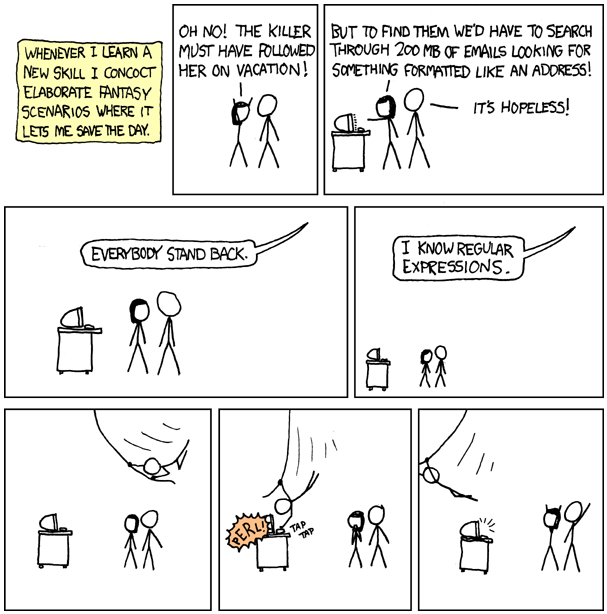
\includegraphics[width=6.4cm]{xkcd208.png}
        \caption*{\tiny  \textcopyright Randall Munroe \href{http://xkcd.com/208/}{xkcd.com} \href{http://creativecommons.org/licenses/by-nc/2.5/}{CC BY-NC 2.5}}
      \end{figure}
    \end{column}    

    %
  \end{columns}
  %
\end{frame}


\begin{frame}[fragile]
  \frametitle{Regular expressions - A case study}
  Formatting street names
  \vspace{0.4cm}
  \begin{minted}{python}
    >>> s = '100 NORTH MAIN ROAD'
  \end{minted}
  \pause
  \vspace{-10pt}
  \begin{minted}{python} 
    >>> s.replace('ROAD', 'RD.')
  \end{minted}
  \pause
  \vspace{-10pt}
  \begin{minted}{python} 
    '100 NORTH MAIN RD.'
  \end{minted}
  \pause
  \vspace{-10pt}
  \begin{minted}{python} 
    >>> s = '100 NORTH BROAD ROAD'
  \end{minted}
  \pause
  \vspace{-10pt}
  \begin{minted}{python}
    >>> s.replace('ROAD', 'RD.') 
  \end{minted}
  \pause
  \vspace{-10pt}
  \begin{minted}{python}
    '100 NORTH BRD. RD.'
  \end{minted}
  \pause
  \vspace{-10pt}
  \begin{minted}{python} 
    >>> s[:-4] + s[-4:].replace('ROAD', 'RD.') 
    '100 NORTH BROAD RD.'
  \end{minted}

  \vspace{0.3cm}
  Better use regular expressions!

  \begin{minted}{python}
    >>> import re 
    >>> re.sub(r'ROAD$', 'RD.', s) 
    '100 NORTH BROAD RD.'
  \end{minted}

  \source{example from Dive Into Python 3 \\ \textcopyright Mark Pilgrim 
    \href{http://creativecommons.org/licenses/by-sa/3.0/}{CC BY-SA 3.0}}

\end{frame}




%%% Local Variables: 
%%% mode: latex
%%% TeX-master: t
%%% End: 
